\section{Sensing}

This section describes the processing of the sensor information to get it into the form needed by the other parts of the system. The data from the laser scanner and the depth information from the RGBD-cameras can be used without significant preprocessing. Therefore this section focuses on the object detection, the room type classification and the doorway detection.

\subsection{Object detection}

The basic idea of this thesis was to create an intelligent system which uses available data to perform the search. Therefore a general object detection system was preferred instead of a specialized one. This is different to most research in this area, where an object detector trained on a few specific objects was used. 

General purpose object detection is a very difficult problem and only the recent success of CNNs in computer vision combined with huge training datasets lead to reasonable solutions. Many of these CNNs including the trained weights are publicly available as they were submitted to computer vision challenges. One of those had to be chosen based on hardware requirements, detectable objects and accuracy.

YOLO was chosen because
\begin{itemize}
 \item there is a version available trained on the COCO dataset and therefore can detect a reasonable number of different object classes. Table \ref{detectable objects} lists the detectable object classes.
 \item it is fast, running with more than 2 frames per second on the used mid-class CPU
 \item it is nearly as accurate as the best solutions and the best of all solutions which run at a reasonable framerate on the used hardware
\end{itemize}

Figure \ref{obj detection} shows a typical result of the object detection, only showing the most likely detections. As one can see the result is far from perfect, especially the confidence is low. This has to be taken into account in the design of the object mapping system, as accumulation of information from multiple images is needed for more reliable results.

\begin{table}
\caption{Detectable object classes}
\begin{tabular}{|l|l|}
\hline
Categories & Classes\\ \hline
Person & Person\\ \hline
Accessory & Backpack, Umbrella, Handbag, Tie, Suitcase\\ \hline
Animal & Bird, Cat, Dog, Horse, Sheep, Cow, Elephant, Bear, \\ & Zebra, Giraffe \\ \hline
Vehicle & Bicycle, Car, Motorbike, Aeroplane, Bus, Train, Truck, \\ &  Boat \\ \hline
Outdoor Objects & Traffic light, Fire hydrant, Stop sign, Parking Meter, \\ &  Bench \\ \hline
Sports & Frisbee, Skis, Snowboard, Sports Ball, Kite, \\ &  Baseball Bat, Baseball Glove, Skateboard, Surfboard, \\ & Tennis Racket \\ \hline
Kitchenware & Bottle, Wine glass, cup, fork, knife, spoon, bowl\\ \hline
Food & Banana, apple, sandwich, orange, broccoli, carrot, \\ &  hot dog, pizza, donut, cake\\ \hline
Furniture & chair, sofa, potted plant, bed, dinig table, toilet\\ \hline
Appliance & Microwave, oven, toaster, sink, refrigerator\\ \hline
Electronics & TV, laptop, mouse, remote, keyboard, cell phone\\ \hline
Indoor Objects & book, clock, vase, scissors, teddy bear, hair drier, \\ &  toothbrush \\ \hline
\end{tabular}
\label{detectable objects}
\end{table}

\begin{figure}[h]
  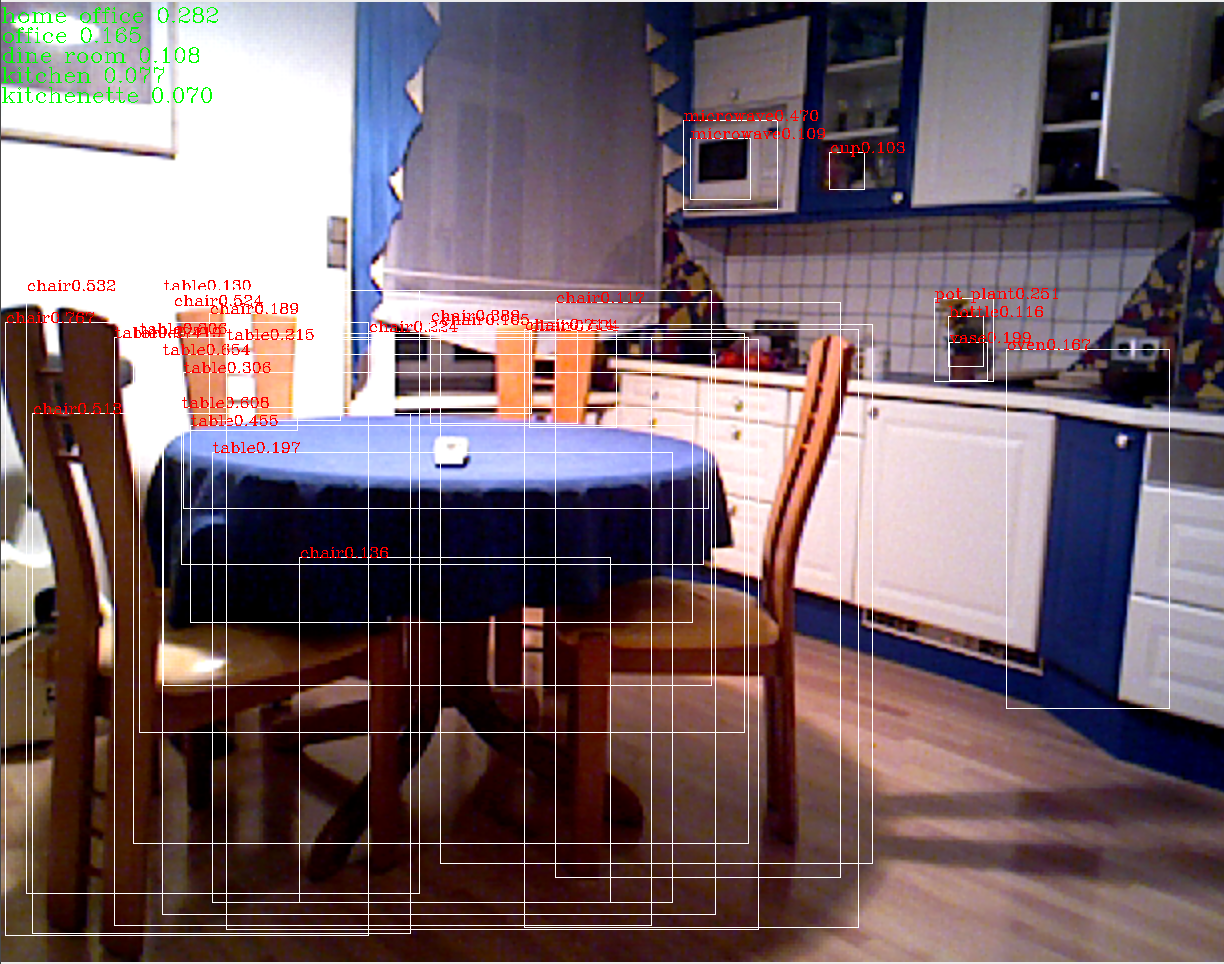
\includegraphics[width=1.0\textwidth]{figures/obj_detection.png}
  \caption{A typical result of the object detection and the place recognition; The bounding boxes together with the most likely class and its probability of the most likely detections are inserted into the image; in the upper left corner of the image the top 5 classification of the place classifier are shown}
  \label{obj detection}
\end{figure}

The problem with this approach is that the result of YOLO is two dimensional bounding boxes whereas in the further processing three dimensional probability distributions of object locations are needed. The RGBD-camera also takes depth images, which contain depth values for every pixel. Due to range limitations and occlusions some pixels may have invalid depth values. Using the depth image every pixel with a valid depth value can be projected into 3D space. However projecting a object detection, represented as a bounding box in 2D, into 3D is much more difficult. A 3D bounding box is not meaningful in many cases, as stray points can be much nearer or further away than the actual object. Fitting a parametric representation is also problematic as they are either not suitable (like a Gaussian) or to costly to compute. 

Therefore a sample-based representation is used. Sample pixels are randomly drawn from the image and projected into 3D. Also information about the enclosing bounding boxes is added to every sample. Samples are drawn from the whole image as also parts of the image without an object have to be represented. Random sampling is used as invalid depth values can be handled easily and regular sampling only makes sense if it is regular in 3D, which is difficult to achieve. The result of the object detection system are a list of all bounding boxes with the corresponding object probabilities and a list of 3D points with additional information about enclosing bounding boxes. 

\subsection{Room type classification}

There are various features which can be used to classify rooms into categories used by humans. Visual features are very expressive for room classification. Another advantage of using images for room type classification is the existence of CNNs trained for place classification due to various computer vision challenges for this task. Therefore such a CNN is used for room type classification. The used classifier is a GoogLeNet CNN trained with 2.5 million images classified into 205 place categories. The network achieves a Top1 accuracy of 0.555 and a Top5 accuracy of 0.857. 

Many of the detectable categories are outdoor place categories. Setting the probabilities of those categories to 0 and renormalizing the other probabilities results in a probability distribution over 82 indoor categories. 

Other features like shape of a room are not used because of their limited expressiveness and the lack of out-of-the-box classifiers. 

\subsection{Doorway detection}

The detection of doorways is important for the segmentation of the environment into rooms. Doorways are narrow passages through walls. Doorways are lower than rooms, usually 2 meters high, and the ceiling of rooms is usually not very cluttered. Therefore the detection was done using point clouds generated by a RGBD-camera looking upwards. The used simple approach classifies space to be a doorway if there is a narrow passage which is about 2 meters high and the space in front and behind the passage is free of obstacles.Sensing.tex